%! TEX root = ../main.tex

\chapter{Evaluación y resultados}
\label{chap:evaluacion}


En este capítulo se detallan las metodologías utilizadas para la evaluación de la 
solución. Estas metodologías están orientadas a valorar los 
aspectos pedagógicos, de diseño, de implementación y de evaluación de la solución 
para determinar su aplicabilidad como herramienta de apoyo al proceso de 
aprendizaje.

%En este capítulo se definen las herramientas diseñadas y utilizadas para evaluar
%la utilización de los juegos serios en el aprendizaje, estas herramientas están
%orientadas a la validación de las hipótesis planteadas en la
%sección~\ref{sec:hipotesis}, así como la evaluación de aspectos pedagógicos, de
%utilidad y de la participación activa del usuario. Estas herramientas se
%utilizan para evaluar a \gls{nombre}.
%
%La evaluación se divide en cinco partes principales:

Las metodologías utilizadas son las siguientes:

\begin{itemize}

    \item \textbf{Prueba preliminar de usabilidad:} es una prueba inicial para
        medir la calidad de la interfaz y la interacción con la misma, esta
        evaluación es realizada con personas no relacionadas al área de
        enfermería, específicamente con alumnos de la carrera de
        Ingeniería en Informática de la \gls{fpuna}.

        La prueba es llevada a cabo durante el desarrollo de la solución a
        diferencia de las demás, las cuales son realizadas una vez terminada la
        solución.

    \item \textbf{Encuesta para determinar la muestra:} es una encuesta acerca del nivel de
        acceso a la tecnología que poseen los alumnos del 4to año  de la carrera 
        de licenciatura en enfermería del \Gls{iab},
        de ahora en más la población objetivo, esta encuesta sirve para definir
        la muestra.

        Se realizar la distribución de \gls{nombre} a los
        alumnos que cumplen con los requisitos mínimos y desean participar de
        las pruebas.%, luego se les realiza la siguientes pruebas para medir su
%        nivel de aceptación y aprendizaje, así como el tiempo y frecuencia de
%        utilización de la solución.

    \item \textbf{Encuesta para evaluar la solución:} es una encuesta realizada
        a cada sujeto de la muestra, donde se busca la opinión del mismo acerca
        de la solución y factores relacionados a la misma. 

    \item \textbf{Encuesta para evaluar conocimiento:} es un cuestionario que es
        completado por la población objetivo, donde se mide el conocimiento de
        los mismos. Con los resultados se busca contrastar el rendimiento de la muestra 
        con respecto a los demás alumnos.
        
        %, se utiliza a los \revisar{También participan} alumnos que
%        no forman parte de la \fixme{muestra}{}, como grupo de control.

%    \item Encuesta para evaluar el conocimiento: es un cuestionario cuyo
%        objetivo es medir el nivel de conocimiento sobre los temas simulados en
%        \gls{nombre}. 
%        
%        La muestra en esta encuesta es la población entera, los alumnos que no
%        utilizaron la aplicación forman un grupo de control.
        
    \item \textbf{Registro de actividades:} es información almacenada por la
        solución automáticamente, y contiene datos acerca del uso y el desempeño
        del alumno.
        
\end{itemize}

Además de describir las metodologías en detalle, también son mostrados y analizados 
los resultados obtenidos en cada una de las evaluaciones realizadas. Los resultados 
son expuestos en forma de tablas y gráficos para mejorar su interpretación.

%El capitulo define los objetivos de la evaluación, describe brevemente conceptos
%transversales a las técnicas utilizadas. Luego, por cada prueba realizada, se
%definen las metodologías, métricas y variables utilizadas en cada parte de la
%evaluación, y se muestran los resultados de las pruebas, al final del capítulo
%se muestran correlaciones entre las variables estudiadas.

\section{Objetivos}


\begin{itemize}
    \item Determinar el nivel de aceptación de la propuesta.
    \item 

\end{itemize}

%! TEX root = ../main.tex

\section{Métricas generales utilizadas en la evaluación}

En esta sección se describen aquellas métricas que son utilizadas por más de una
metodología para la evaluación de la solución, las cuales se consideran que son
importantes detallar.

Una de estas métricas es la escala de \textit{Likert}, la cual es una métrica
utilizada en la \emph{Encuesta para evaluar la solución} y en la encuesta
correspondiente a la \emph{Prueba preliminar de usabilidad}. Otra métrica
utilizada es la correlación de \textit{Pearson}, esta métrica es utilizada para
medir el grado de relación entre variables de las encuestas realizadas, los
registros de actividades, entre otros.

Cabe destacar que en~\cite{norman2010likert} se demuestra que, aunque el tamaño
de la muestra sea pequeña y los datos no puedan ser distribuidos normalmente o
los datos sean de escalas de tipo \textit{Likert}, los métodos paramétricos como
el análisis de varianza, la regresión y la correlación pueden ser utilizados.


\subsection{Escala de Likert}
\label{sec:likert}

Para la valoración de las variables medidas en la \emph{Prueba preliminar de
    usabilidad} y la {Encuesta para evaluar la solución} se utiliza la escala de
\textit{Likert}\cite{Allen:2007} de 7 valores posibles. La escala de
\textit{Likert} es utilizada para permitir a las personas indicar cuánto están
de acuerdo o en desacuerdo con respecto a ciertos puntos. Los valores
utilizados, son:

\begin{enumerate}
    \item Totalmente en desacuerdo.
    \item En desacuerdo.
    \item Parcialmente en desacuerdo.
    \item Neutral.
    \item Parcialmente de acuerdo.
    \item De acuerdo.
    \item Totalmente de acuerdo.
\end{enumerate}

Una vez valoradas y registradas todas las respuestas y con el objetivo de
eliminar las tendencias en la forma en la que son completadas las
encuestas\cite{Fischer2010} se utiliza el método de \emph{Doble Estandarización}
recomendado en~\cite{Pagolu2011}. Este método, consiste en dos
estandarizaciones, la primera por fila, que en este caso representa a los
individuos y la segunda por columna donde cada columna representa una de las
diferentes preguntas de la encuesta.

Siendo:
\begin{itemize}
	\item $\min_i$ la respuesta de menor valor del usuario $i$.
	\item $\max_i$ la respuesta de mayor valor del usuario $i$.
\end{itemize}

Para cada respuesta $s$ del usuario $i$, el valor ajustado, por la primera
normalización, $s_1$ se define como:

\begin{equation}
s_1{_i}=\frac{s-\min_i}{\max_i-\min_i}
\end{equation}

%\observacion{Considerar resumir}
Y luego siendo:
\begin{itemize}
	\item $groupmin_i$ la respuesta ajustada de menor valor en el grupo $i$.
	\item $groupmax_i$ la respuesta ajustada de mayor valor en el grupo $i$
\end{itemize}

Para cada respuesta ajustada $s_1{_i}$ del usuario $i$, el valor ajustado $sa_i$ se
define como:	

\begin{equation}
sa_i=\frac{s_{1_i}-groupmin_i}{groupmax_i-groupmin_i}
\end{equation}

Obteniendo así un valor normalizado, tanto por individuo, como por pregunta, en
el rango $0$ y $1$.

Para la valoración absoluta de cada  item se utiliza la media de cada columna o
respuesta a una pregunta de la encuesta.

Siendo:
\begin{itemize} 
\item $r_{k_i}$ la respuesta del usuario $i$ a la pregunta $k$.
\item $t_k$ la cantidad total de usuarios que respondieron la pregunta $k$.
\end{itemize}

El puntaje promedio de cada pregunta o item evaluado  $p_k$ en la encuesta se
define como:

\begin{equation}
p_k = \frac{\sum_{i=1}^n{r_{k_i}}}{t_k}
\end{equation}

%\subsubsection{Manejo de información faltante}
%\label{sec:informacion_faltante}
%\observacion{No repetir tanto existe}
%
%En toda encuesta pueden haber preguntas que no son respondidas por los encuestados, 
%en este tipo de situaciones existen tres posibles formas de categorizar el 
%patrón de ocurrencia de la falta de 
%respuestas\cite{leite2010performance,tsikriktsis2005review}:
%
%\begin{description}
%    \item[Información faltante completamente aleatoria:] cuando la información
%        faltante es independiente de la variable medida y de otras variables.
%    \item[Información faltante aleatoria:] cuando la información faltante depende
%        de otras variables, pero no de la variable en sí. 
%    \item[Información faltante no aleatoria:] cuando hay una relación entre la
%        información faltante y el valor de la variable.
%\end{description}
%
%Una vez categorizado el patrón de ocurrencia, existen a su vez tres
%mecanismos~\cite{tsikriktsis2005review} principales para lidiar con información
%faltante como son la eliminación, el reemplazo y los  procedimientos basados en
%modelo.~\cite{tsikriktsis2005review} recomienda utilizar un mecanismo de
%reemplazo para escalas del tipo \textit{Likert}.
%
%Las técnicas de reemplazo se clasifican en tres grandes
%grupos\cite{tsikriktsis2005review}:
%\begin{enumerate*}[label=\itshape\alph*\upshape)]
%\item basadas en el promedio,
%\item basadas en regresión, e,
%\item imputación \emph{hot deck}.
%\end{enumerate*}
%
%\fixme{De estas técnicas se seleccionó la sustitución}{Resaltar}. Basada por
%promedio ya que las relaciones entre las variables son bajas y los datos
%faltantes son menos del $10\%$. La sustitución basada por promedio se divide
%nuevamente en tres grupos\cite{tsikriktsis2005review}; promedio
%\begin{enumerate*}[label=\itshape\alph*\upshape.]
%\item total,
%\item del subgrupo, y,
%\item por caso.
%\end{enumerate*}
%
%La sustitución por promedio total es elegida debido a que la relación entre la
%variable que falta y las demás variables en los datos es relativamente baja, es
%fácil de usar y retiene la muestra. La sustitución por promedio total se realiza
%obteniendo el promedio de todas las respuestas de la pregunta cuya respuesta
%falte, la sustitución de subgrupo es similar, solo que se limita a aquellos
%sujetos del mismo subgrupo del sujeto que no respondió, y finalmente, la
%sustitución por caso, es el promedio de las respuestas válidas del sujeto.

\subsection{Correlación de variables aleatorias}
\label{sec:def_correlacion}

Las correlaciones se utilizan durante una etapa exploratoria o de observación de
la investigación para determinar las variables que tienen al menos una relación
estadística con cada uno de los diseños experimentales. Las correlaciones
también se utilizan para determinar el grado de asociación entre variables
dependientes e independientes. Por otro lado, el coeficiente de correlación se
utiliza comúnmente para cuantificar el grado de asociación entre dos variables
\cite{BoslaughStatistics2008}.

La correlación de Pearson\cite{BoslaughStatistics2008} mide la relación que
existe entre dos variables, $X$ e $Y$, el mismo esta comprendido entre $-1$ y
$1$, en su punto más bajo ($-1$) indica que una de las dos variables crece
mientras la otra decrece, y en su punto más alto ($1$), indica que ambas crecen
o decrecen conjuntamente, el valor $0$, indica que no existe una relación entre
ambas variables.

El coeficiente para las variables $X$ e $Y$ está dado por:

\begin{equation}
r = \frac{\sum_{i=1}^n{(\frac{x_i-\bar{x}}{s_x})({\frac{y_i-\bar{y}}{s_y}})}}%
{n - 1}
\end{equation}

donde:

\begin{itemize}
    \item ($x_i$, $y_i$) es el conjunto de coordenadas de las variables $X$ e $Y$.
    \item $\bar{x}$ es la media de la variable $X$.
    \item $\bar{y}$ es la media de la variable $Y$.
    \item $s_x$ es la desviación estándar de la variable $X$.
    \item $s_y$ es la desviación estándar de la variable $Y$.
    \item $n - 1$ son los grados de libertad.
\end{itemize}

%! TEX root = ../main.tex

\section{Prueba preliminar de usabilidad}
\label{sec:interfaz}

Durante el desarrollo de la solución se realizó una prueba para evaluar la 
interfaz de usuario, específicamente buscando la retroalimentación de usuarios 
acostumbrados a tecnología similar a la utilizada en la solución.

Esta prueba ayuda en el proceso de diseño e implementación de la solución con 
las características mencionadas en los objetivos del trabajo y acorde a los 
requerimientos. De esta manera se pueden identificar los aspectos que deben 
ser mejorados.

La prueba consta de dos partes importantes involucradas en la recolección
de datos para su posterior análisis. Estas partes son las siguientes:

\begin{description}

\item[Simulación:] luego de una explicación acerca de las funciones y manejos
    generales de la solución por parte de los encargados de la prueba, cada usuario
    completa una tarea que consiste en realizar el procedimiento de venopunción con la 
    solución, como ayuda, recibe una hoja con una lista de todos los pasos 
    necesarios para llevar a cabo el procedimiento.
    	
    Las simulaciones son grabadas con programas de captura de pantalla, así
    como por detectores de eventos táctiles.
    	
\item[Encuesta:] posteriormente se le provee una encuesta a cada
    usuario la cual es utilizada para obtener una idea general acerca de la
    calidad de la simulación según la percepción de los usuarios. Esta encuesta 
    contiene preguntas que son medidas mediante la escala de tipo Likert. 

\end{description} 

\subsection{Muestra}

La prueba de usabilidad de la interfaz de usuario se realiza con alumnos de la carrera de
Ingeniería en Informática de la \Gls{fpuna}, sin experiencia previa tanto con la
solución como con los procedimientos simulados, pero sí familiarizados con la
utilización de dispositivos móviles. La muestra no requiere de sujetos que sean
parte del \emph{población objetivo} ya que sólo está
orientada a mejorar aspectos de interfaz de usuario y no el contenido de la
solución, además se considera que la muestra puede brindar una evaluación más
crítica debido a su familiarización con interfaces similares a la de la
solución.

El número de muestras tomadas fue 8, ya que según~\cite{nielsen2000} son
necesarios al menos $5$ participantes para poder obtener resultados
significativos en una prueba de usabilidad. Además,~\cite{ritch2009} asegura que
la teoría de~\cite{nielsen2000} es verdadera especialmente para pruebas simples. 

Se fundamenta el número de participantes, y que es una prueba sencilla, ya que:

\begin{itemize}

\item La prueba no debería tomar más de $10$ minutos en ser realizada.

\item Se busca solamente obtener información acerca de la interfaz, y no el
    funcionamiento en sí de la simulación, pues los usuarios no son expertos en
    el área y no tienen conocimiento acerca las tareas.

\item No se busca evaluar el aspecto pedagógico de la solución sino sólo su interfaz gráfica.
%\item No se busca medir el aprendizaje del usuario en temas no relacionados a la
%    interfaz, es decir, no se mide el aprendizaje del usuario en el tema
%    simulado\revisar{No se entiende, no se mide el aspecto pedagógico solo la
%    interfaz gráfica de la simulación}.

\item El procedimiento de enfermería a realizarse con la solución está bien definido 
y los pasos necesarios están a disposición del usuario en todo momento.

\end{itemize}

\subsection{Variables}
\label{sec:evaluacion_interfaz_variables}

Antes de definir las variables, se deben primero definir los conceptos 
relacionados a los tipos de acciones que pueden realizarse sobre el paciente 
virtual en la solución, los mismos son:

%\observacion{Cual se encarga del diseño de la simulación?}
\begin{itemize}
\item \textbf{Acción por menú contextual:} se refiere a las acciones que el usuario 
    puede realizar utilizando el menú contextual que aparece sobre cada uno de los elementos 
    disponibles en la solución.
\item \textbf{Acción por menú de la \Gls{gui}:} se refiere a las 
    acciones que el usuario puede realizar seleccionando una opción en los menús 
    principales que presenta la interfaz de la solución.
\item \textbf{Acción con elemento:} se refiere a las actividades que el usuario 
    puede realizar cuando tiene seleccionado un elemento y que no involucre el 
    uso del menú contextual.
\end{itemize}


Las variables medidas durante la realización de la tarea con la solución son las
siguientes:

%\observacion{No repetir tanto la descripción en el título}

\begin{itemize}

\item \textbf{Tiempo de realización de la primera acción por tipo:} cuanto tiempo 
	le toma al usuario realizar la primera vez una acción agrupado por tipo (por menú 
	contextual, por menú de la \Gls{gui}, con elementos).

%\item \textbf{Tiempo de realización de la primera acción por menú contextual:} 
%    cuanto tiempo le toma al usuario realizar una acción por menú contextual la 
%    primera vez.
%
%\item \textbf{Tiempo de realización de la primera acción por \Gls{gui}:} cuanto 
%    tiempo le toma al usuario realizar una acción por menú de 
%    interfaz gráfica de usuario la primera vez.
%    
%\item \textbf{Tiempo de realización de la primera acción por herramienta:} cuanto 
%    tiempo le toma al usuario realizar una acción por herramienta la primera vez.

\item \textbf{Tiempo de realización de las siguientes acciones por tipo:} cuanto tiempo 
	le toma al usuario realizar las siguientes veces una acción agrupado por 
	tipo (por menú contextual, por menú de la \Gls{gui}, con elementos).
 
%\item \textbf{Tiempo de realización de las siguientes acciones por menú contextual:} 
%    cuanto tiempo le toma al usuario realizar una acción por menú 
%    contextual las siguientes veces.
%
%\item \textbf{Tiempo de realización de las siguientes acciones por \Gls{gui}:} 
%    cuanto tiempo le toma al usuario realizar una acción 
%    por interfaz gráfica de usuario las siguientes veces.
%
%\item \textbf{Tiempo de realización de las siguientes acciones por herramienta:} 
%    cuanto tiempo le toma al usuario realizar una acción por herramienta 
%    las siguientes veces.

\item \textbf{Tiempo total:} se refiere al tiempo empleado por el usuario para 
    completar la tarea asignada.

\item \textbf{Número de pasos realizados:} cantidad de pasos requeridos en la tarea 
    que son realizados por el usuario en la simulación. 

\item \textbf{Cantidad de movimientos espaciales por tipo:} número de veces en que se 
    modifica el estado de la cámara para realizar las acciones deseadas agrupados por 
    tipo (desplazamiento, acercamiento/alejamiento).

%    \observacion{Esto donde entra?}

\end{itemize}

En cuanto a la encuesta, las siguientes son las variables que fueron consideradas 
y medidas:

\begin{itemize}

\item \textbf{Calidad gráfica:} realismo y calidad de los modelos utilizados.

\item \textbf{Interacción:} desenvolvimiento en el entorno y utilización del 
    hardware.

\item \textbf{Interacción con objetos:} utilización errónea de objetos.

\item \textbf{Características del entorno:} realismo del escenario y de los 
    objetos utilizados.

\item \textbf{Usabilidad de la interfaz:} facilidad de uso de las opciones 
    proveídas por la interfaz.

\item \textbf{Integración con el hardware:} facilidad de uso de la solución con 
    un dispositivo móvil. 

\end{itemize}

\subsection{Métricas}

Para la medición de las variables relacionadas a la encuesta,  se utiliza la escala
de Likert con la \emph{Doble estandarización} explicada en la
sección~\ref{sec:likert}. 

En cambio, para la medición de las variables relacionadas a la interacción del usuario con 
la solución se utilizan las grabaciones registradas durante las pruebas y las
las siguientes métricas:

%Para el análisis de la encuesta realizada a los usuarios, se utiliza la escala
%de Likert con la \emph{Doble estandarización} explicada en la
%sección~\ref{sec:likert}, y en el análisis de la interacción del usuario con la
%solución se utilizan las grabaciones registradas durante la prueba.
%
%Haciendo uso de las variables descriptas anteriormente, las métricas
%utilizadas son las siguientes:

\begin{itemize}
    
\item \textbf{Tiempo promedio de realización de las siguientes acciones por menú contextual:} 
    se obtiene dividiendo la cantidad total de tiempo empleado en realizar acciones por menú 
    contextual por el número de veces que se realizaron esas acciones, sin considerar la primera 
    vez. 
    
\item \textbf{Tiempo promedio de realización de las siguientes acciones por \Gls{gui}:} 
    se obtiene dividiendo la cantidad total de tiempo empleado en realizar acciones por \Gls{gui} 
    por el número de veces que se realizaron esas acciones, sin considerar la primera 
    vez. 
    
\item \textbf{Tiempo promedio de realización de las siguientes acciones por herramienta:} 
    se obtiene dividiendo la cantidad total de tiempo empleado en realizar acciones por 
    herramienta por el número de veces que se realizaron esas acciones, sin considerar la 
    primera vez. 
    
\item \textbf{Promedio de pasos correctos:} se obtiene dividiendo la cantidad de 
    pasos requeridos realizados por los usuarios sobre la cantidad de pasos requeridos. 
    
\item \textbf{Promedio de movimientos por tipo:} se obtiene dividiendo el número de 
    movimientos que fueron realizados agrupados por tipo (desplazamiento, acercamiento/
    desplazamiento) por la cantidad de usuarios.
    
\item \textbf{Promedio del tiempo total:} se obtiene dividiendo el tiempo total empleado 
    por los usuarios para completar la tarea asignada por el número de usuarios.

\end{itemize}

\subsection{Resultados obtenidos}
\label{sec:res_interfaz}

A continuación de muestran y analizan los resultados obtenidos en la prueba. Los resultados 
se dividen en \emph{simulación} y \emph{encuesta} para una mejor comprensión.

\subsubsection{Simulación}

Las grabaciones realizadas a las sesiones de los usuarios se utilizan para medir
el grado de facilidad de aprendizaje de la interfaz de usuario.

Dados los tres tipos de acciones descritos en~\ref{sec:evaluacion_interfaz_variables}, la
tabla~\ref{tab:interfaz_tiempo_acciones} muestra el tiempo, en segundos,
que le tomo a cada usuario realizar una acción la primera vez y 
el tiempo que les tomo en promedio las demás veces, para cada uno de los tipos 
de acciones.

%\observacion{Hacer énfasis en la comparación entre el primer y los siguientes}

\begin{table}[!hbt]
\centering
\begin{tabular}{|c|c|c|c|c|c|c|}
\hline
\rowcolor{gris} \textbf{} & \multicolumn{2}{|c|}{\textbf{Menú Contextual}} &
\multicolumn{2}{|c|}{\textbf{Menú de la Interfaz}} &
\multicolumn{2}{|c|}{\textbf{Herramienta}}\\
\hline
\rowcolor{gris} Usuario & Primera & Siguientes & Primera & Siguientes & Primera & Siguientes \\
\hline 1 &  8 &  2.25 &  3 & 9.14 & 11 & 3.0 \\
\hline 2 & 30 &  7.00 &  4 & 3.57 &  7 & 4.5 \\
\hline 3 &  5 &  2.25 &  5 & 1.86 &  1 & 1.0 \\
\hline 4 &  2 & 13.00 &  4 & 2.00 &  1 & 0.5 \\
\hline 5 & 18 &  2.75 &  6 & 4.43 &  6 & 3.0 \\
\hline 6 &  4 & 14.25 & 11 & 7.86 & 13 & 4.0 \\
\hline 7 &  5 &  8.00 &  4 & 4.71 & 20 & 2.5 \\
\hline 8 &  3 &  2.33 & 10 & 3.57 &  3 & 6.5 \\
\hline
\textbf{Promedio} & 9.38 & 6.37 & 5.88 & 4.64 & 7.75 & 3.125 \\
\end{tabular}
\caption{Tiempo por acciones la primera vez y las siguientes veces que se realizo}
\label{tab:interfaz_tiempo_acciones}
\end{table}

En la tabla~\ref{tab:interfaz_tiempo_acciones} se observa consistentemente una 
mejora en el tiempo de realización de un tipo de acción con respecto a la primera vez 
que es realizada. 

En la figura~\ref{fig:interfaz_tiempo_acciones} se observa como en promedio el
usuario aprende, y en las siguientes acciones similares demora menos tiempo,
este es un factor importante y es el objetivo de esta prueba pues muestra que la
interfaz es fácil de usar, y con tres tipos de acciones, el usuario puede
utilizarla sin mayores inconvenientes. Se observa una mejoría del $30\%$ en las
\emph{Acciones por menú contextual}, $21\%$ en las \emph{Acciones por menú de la
    \Gls{gui}} y finalmente, una mejoría del $60\%$ en las \emph{Acciones con elementos}.

%\begin{figure}[H]
%\centering
%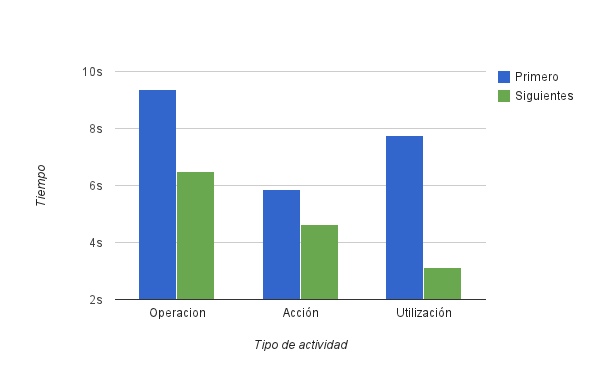
\includegraphics[width=14cm]{resultados/imagenes/interfaz_tiempo_actividades.png}
%\caption{Tiempo por tipo de actividad}
%\label{fig:interfaz_tiempo_acciones}
%\end{figure}

\begin{filecontents}{interfazuso.dat}
n   p       s
1	9.38	6.48
2   5.88	4.64
3   7.75	3.13
\end{filecontents}
\pgfplotstableread{interfazuso.dat}{\InterfazUso}

\begin{figure}[H]
    
        \centering
        \begin{tikzpicture}[scale=1]
           \begin{axis}[ybar,%
              legend pos=outer north east,
              xmin=1,
              xmax=3,
              x=2.5cm,
              enlarge x limits={abs=1cm},
              xtick=data,
              symbolic x coords={0,1,2,3,4},
              ymin=0,ymax=10,
              %ytick={0,2,4,6,8,10},
              xticklabels={Contextual,Interfaz,Herramienta},
              ylabel= Tiempo (s),
              xlabel= Tipo de acción,
              bar width=10pt,
              %enlarge x limits={abs=2},
                ]   
        \addplot[color=blue,ybar,fill=blue!75,area legend] table [x = {n}, y = {p}] {\InterfazUso};
        \addlegendentry{Primer}
        \addplot[color=red,ybar,fill=red!75,area legend] table [x = {n}, y = {s}]
        {\InterfazUso};
        \addlegendentry[align=left]{Promedio \\ siguientes}
        \end{axis}
        \end{tikzpicture}
        \caption{Tiempo por tipo de acción}
        \label{fig:interfaz_tiempo_acciones}
\end{figure}

En la tabla~\ref{tab:interfaz_cantidad_espaciales} se observa la cantidad de
movimientos espaciales realizados por los usuarios, se observa que en promedio
se desplazaron $10,88$ veces por el escenario, y $6,75$ veces acercaron o
alejaron la cámara del paciente.

%\observacion{Hay que dejar bien en claro de donde sale esto, por que es
%importante entender el significado de esta diferencia}

\begin{table}[H]
\centering
\begin{tabular}{lrrr}
\toprule
\textbf{Jugador}  & \textbf{Desplazamiento} & \textbf{Acercamiento/alejamiento} & \textbf{Total} \\
\midrule
1        & 18         & 2    & 20 \\
2        & 7          & 8    & 15 \\
3        & 14         & 12   & 26 \\
4        & 9          & 14   & 23 \\
5        & 5          & 8    & 13 \\
6        & 14         & 4    & 18 \\
7        & 16         & 3    & 19 \\
8        & 4          & 3    &  7 \\
\midrule
\textbf{Promedio} & \textbf{10,88}      & \textbf{6,75} & \textbf{17,63} \\
\bottomrule
\end{tabular}
\caption{Cantidad de movimientos espaciales}
\label{tab:interfaz_cantidad_espaciales}
\end{table}

No existe una cantidad mínima o máxima de movimientos que el usuario debe realizar para acercar, 
alejar o desplazar la cámara. Los datos mostrados en la tabla~\ref{tab:interfaz_cantidad_espaciales} 
muestran que no son necesarias demasiados movimientos. Teniendo en cuenta esta información y la 
proveída en la tabla~\ref{tab:interfaz_tiempo_total}, se concluye 
que en promedio los usuarios realizan $1,7$ movimientos por minuto.

\begin{table}[!hbt]
\centering
\begin{tabular}{lrrr}
\toprule
\textbf{Alumno} & \textbf{Tiempo (min)} \\
\midrule
1        & 8:32 \\
2        & 6:03 \\
3        & 8:33 \\
4        & 5:17 \\
5        & 6:55 \\
6        & 8:40 \\
7        & 7:03 \\
8        & 10:27 \\
\midrule
\textbf{Promedio} & \textbf{7:41} \\
\bottomrule
\end{tabular}
\caption{Tiempo de prueba por usuario}
\label{tab:interfaz_tiempo_total}
\end{table}

El tiempo total que se observa en la tabla~\ref{tab:interfaz_tiempo_total},
muestra que en promedio a cada alumno le tomo $7:41$ minutos realizar todos los
pasos especificados, es importante notar que este tiempo incluye el tiempo de
adaptación. 

La tabla~\ref{tab:interfaz_acciones} nos muestra la cantidad de pasos
realizados por los alumnos de un total de 19. Se observa que en promedio 
realizaron $16.75$ pasos.
%esto permite identificar en que parte del procedimiento los usuarios tienen
%inconvenientes en cuanto al uso de la interfaz.

\begin{table}[H]
\centering
\begin{tabular}{lrrr}
\toprule
\textbf{Alumno} & \textbf{Pasos realizados (19)} \\
\midrule
1 & 19 \\
2 & 15 \\
3 & 18 \\
4 & 15 \\
5 & 18 \\
6 & 16 \\
7 & 19 \\
8 & 14 \\
\midrule
\textbf{Promedio} & \textbf{16,75} \\
\bottomrule
\end{tabular}
\caption{Pasos realizados por alumno}
\label{tab:interfaz_acciones}
\end{table}



\subsubsection{Encuesta}


La encuesta es utilizada para obtener el grado de
disconformidad de los usuarios con respecto a la solución. Se utiliza la disconformidad 
para resaltar los puntos débiles, así, aquellas variables que tengan el mayor porcentaje serán
las que deban ser mejoradas.

%Las preguntas que forman parte de la  encuesta son agrupadas en cuanto a
%aspectos de calidad gráfica, interacción con el entorno, interacción con los
%objetos, características del entorno, usabilidad de la interfaz e integración
%con el hardware.

En la tabla~\ref{tab:interfaz_disconformidad_metrica} se observan que las mayores 
disconformidades son la usabilidad de la interfaz de usuario que llega al $51\%$, la 
interacción de los usuarios con el entorno que llega al $50\%$ y la interacción con los 
objetos que llega al $49\%$. Otras disconformidades con menor porcentaje son las
características del entorno con un  $33\%$, la integración con el hardware con
un $27\%$ y por último la calidad gráfica con un $17\%$.

%\observacion{Hay que explicar que estas pruebas se hicieron de forma previa a
%las demás y que se arreglan algunos casos}

\begin{table}[H]
\centering
\begin{tabular}{lr}
\toprule
Variable & Disconformidad (0-1)\\
\midrule
Calidad Gráfica         & 0.17 \\
Interacción Entorno     & 0.50\\
Interacción Objetos     & 0.49\\
Características Entorno & 0.33\\
Usabililidad Interfaz   & 0.51\\
Integración Hardware    & 0.27\\
\bottomrule
\end{tabular}
\caption{Disconformidad por variable}
\label{tab:interfaz_disconformidad_metrica}
\end{table}

%La conclusión de esta prueba de interfaz, es que si bien, pudo ser utilizada sin
%mayores inconvenientes, existe un alto grado de disconformidad con la interfaz,
%además cabe resaltar, los sujetos de prueba son personas acostumbradas al uso de
%tecnologías similares. Otros puntos débiles encontrados en esta prueba son la
%interacción con el entorno y  con los objetos.

Como consecuencia de los resultados obtenidos, la usabilidad de interfaz y la interacción con objetos y 
con el entorno son mejoradas para obtener la versión final de la solución que es utilizada por 
los estudiantes de enfermería. Las demás pruebas mencionadas en este capítulo son realizadas con 
la versión final de la solución.
%elementos sufren modificaciones a fin de su utilización con usuarios no
%técnicos.

%Las demás pruebas mencionadas en este capítulo son realizadas con la versión
%final de la solución, la cual es obtenida luego de las mejoras realizadas a los
%puntos débiles detectados por esta prueba.

%! TEX root = ../main.tex

\section{Encuesta de ubicación}
\label{sec:ubicacion}

Para recabar información acerca del nivel de acceso  de los alumnos a la
tecnología, se realiza una encuesta que cuenta con diez preguntas, las cuales
buscan conocer el modelo de dispositivo móvil, el acceso a
Internet, y la predisposición de cada alumno a ayudar en la prueba.

Con los resultados de la encuesta de ubicación tecnológica, se seleccionan
aquellos alumnos que poseen dispositivos móviles que superan o igualan las
especificaciones descritas más adelante. De esta encuesta se obtendrán los 
usuarios que formarán parte de la población que evaluará la versión final de 
la solución.

\subsection{Muestra}

En el año $2014$, el \Gls{iab} cuenta con $124$ alumnos en el cuarto año  de la 
carrera de Licenciatura en Enfermería distribuidos en
tres secciones, estos alumnos son considerados la población objetivo. De los 124, 93 de
ellos estuvieron interesados en completar la encuesta.

\subsection{Variables}

Se definen $3$ factores necesarios para que un alumno pueda ser considerado como
sujeto de prueba, el primero es la predisposición del mismo a participar de la
prueba, el segundo es que posea un dispositivo móvil que supere los requisitos
mínimos explicados más adelante y el tercero es que tenga algún tipo de conexión a 
internet desde el dispositivo móvil pues 
los registros de actividad de cada dispositivo deben ser enviados y almacenados 
para su posterior interpretación y análisis. A continuación se describen las variables 
consideradas.


\begin{itemize}

\item \textbf{Requisitos mínimos:} son aquellos requerimientos técnicos con los que 
    debe cumplir completamente el dispositivo móvil del usuario para que la 
    solución tenga un desempeño que garantice una experiencia fluida a la hora de 
    utilizarla. Estos requisitos son:
    \begin{itemize}
        %%\item Sistema Operativo Android $4.0$ o superior
        \item Memoria ram de $512$MB o superior.
        \item Velocidad de procesador de $800$ GHz o superior.
        \item \Gls{gpu} OpenGL ES 2.0 o superior.
        %\item Conexión frecuente a internet.
    \end{itemize}
    Los requisitos de \textit{hardware} mencionados, son requeridos por las
    características de la simulación, una \Gls{gpu} es requerida por los gráficos en 
    tres dimensiones.

\item \textbf{Tipo de acceso a internet:} el tipo de acceso a internet que posee el 
    usuario en su dispositivo móvil. Puede ser una de las siguientes opciones:
    plan post-pago, paquetes pre-pago, acceso ocasional y sin acceso.
    
\item \textbf{Sistema Operativo:} se refiere al tipo de sistema operativo que posee 
    el dispositivo móvil del usuario.

%    \observacion{Donde se menciona?}
    
\end{itemize}

\subsection{Métricas}

Las métricas utilizadas para estudiar los datos recogidos son sencillas ya que
sólo buscan determinar la población que evaluará la solución, estas métricas son
las siguientes:

\begin{itemize}
\item Porcentaje de encuestados con dispositivos móviles que cumplen y que no cumplen con 
los requisitos mínimos.
\item Porcentaje del tipo de acceso a internet de los encuestados desde sus dispositivos móviles.
\item Porcentaje del tipo de sistema operativo que poseen los dispositivos móviles de los 
encuestados.
\end{itemize}


\subsection{Resultados obtenidos}


%Como se indicó en la sección~\ref{sec:ubicacion}, se agrupa a los
%\fixme{alumnos}{De donde?} encuestados de acuerdo a las características de sus
%dispositivos móviles y del acceso a internet.

%El acceso a internet es un requisito importante, pues para que los mismos puedan
%enviar su progreso y así se registre la utilización de la solución, así, es
%necesario que los usuarios tengan un acceso ocasional a internet. 

En la figura~\ref{fig:ubicacion_acceso_internet} se puede observar que de 93 alumnos 
encuestados, el $94,6\%$ tiene acceso a internet al menos en algún momento y que
solo el $5.4\%$ no tiene acceso a internet en sus dispositivos móviles. Considerando 
sólo estos datos, el $94,6\%$ de los alumnos podría utilizar la solución.

%esto
%permite que tengan acceso a la solución el $94,6\%$ de los alumnos.

%\begin{figure}[H]
%\centering
%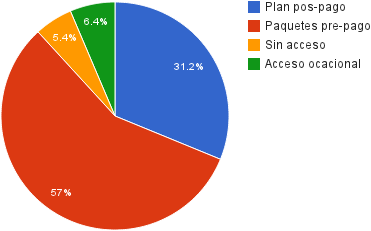
\includegraphics[scale=0.5]{resultados/imagenes/ubicacion_acceso_internet.png}
%\caption{Acceso a internet desde dispositivos móviles}
%\label{fig:ubicacion_acceso_internet}
%\end{figure}

 \begin{figure}[H]
        \centering
        \begin{tikzpicture}[thick,scale=0.7, every node/.style={transform shape}]
            \pie[
                %explode=.2,
                text=legend,
                %style=drop shadow,
                %radius=3,
                %scale font,
                explode={0.1,0.1,0.3,0.3}
                ]%
            {%
                31.2 / Plan pos-pago,
                57   / Paquetes pre-pago,
                5.4  / Sin acceso,
                6.4  / Acceso ocasional}
        \end{tikzpicture}
        \caption{Acceso a internet desde dispositivos móviles}
        \label{fig:ubicacion_acceso_internet}
\end{figure}

%La utilización en dispositivos móviles es un requisito necesario para
%\fixme{la}{Utilizar la solución} solución

Los dispositivos móviles son un requisito para utilizar la solución, 
en la figura\ref{fig:ubicacion_sistemas_operativos} se muestran los sistemas operativos
móviles utilizados por los alumnos encuestados, si bien el motor de videojuego 
utilizado permite generar clientes a diversos sistemas operativos, es importante conocer el sistema
operativo que poseen los alumnos para realizar pruebas.

En la figura~\ref{fig:ubicacion_sistemas_operativos} se puede observar que
\emph{Android} lidera con un $61.3\%$, le sigue Windows Phone con un $12.9\%$.
Si bien, según la tabla~\ref{tab:comparacion_motores_juegos}, \emph{Unity3D}
soporta la mayoría de los sistemas operativos, aún es importante hacer pruebas
sobre un sistema operativo específico. Se selecciona \emph{Android} por ser el
sistema operativo con mayor cuota entre los alumnos.

%\begin{figure}[H]
%\centering
%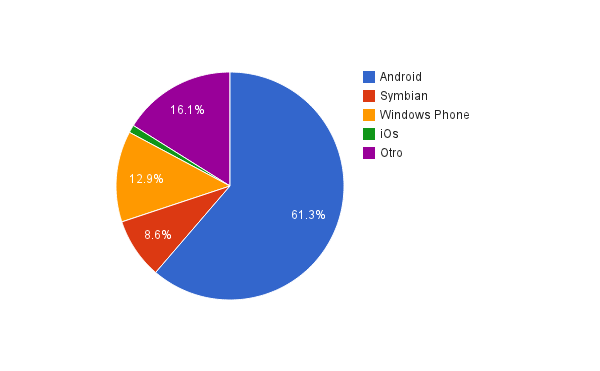
\includegraphics[scale=0.5]{resultados/imagenes/ubicacion_sistemas_operativos.png}
%\caption{Sistemas operativos móviles utilizados}
%\label{fig:ubicacion_sistemas_operativos}
%\end{figure}

 \begin{figure}[H]
        \centering
        \begin{tikzpicture}[thick,scale=0.7, every node/.style={transform shape}]
            \pie[
                text=legend,
                rotate=61.3,
                explode={.1,.2,.2,.2}
                ]%
            {%
            61.3 / Android,
             8.6 / Symbian,
            12.9 / Windows Phone,
            17.2 / Otros}
        \end{tikzpicture}
        \caption{Sistemas operativos móviles utilizados}
	    \label{fig:ubicacion_sistemas_operativos}
\end{figure}
    

Por último, se divide a los encuestados para determinar cuantos de ellos
tiene dispositivos móviles que cumplen los requisitos mínimos para utilizar la
solución propuesta según lo descrito en la sección~\ref{sec:ubicacion}. En la
figura~\ref{fig:ubicacion_requisitos_minimos} se puede observar que el $18,3\%$
de los encuestados cumplen con los requisitos.

Si bien los requisitos de la solución no son elevados para los estándares
actuales, la figura~\ref{fig:ubicacion_requisitos_minimos} nos muestra que el
$18.3\%$ tiene dispositivos de alta gama, el cual es un porcentaje mayor al
esperado. Se observa además que cerca del
$90\%$ posee un dispositivo de gama media o superior, la penetración de los
dispositivos móviles es muy alta en los estudiantes de enfermería del \Gls{iab}.

%\begin{figure}[H]
%\centering
%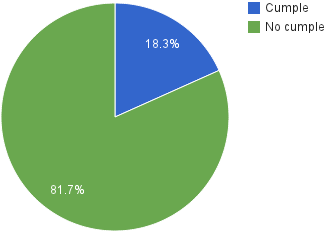
\includegraphics[scale=0.5]{resultados/imagenes/ubicacion_requisitos_minimos.png}
%\caption{Dispositivos que cumplen con los requisitos mínimos para la prueba}
%\label{fig:ubicacion_requisitos_minimos}
%\end{figure}

\begin{figure}[H]
       \centering
       \begin{tikzpicture}[thick,scale=0.7, every node/.style={transform shape}]
           \pie[
                text=legend,
                explode=.1
                ]%
            {%
                81.7 /  No Cumple,
                18.3 /  Cumple
            }
        \end{tikzpicture}
        \caption{Dispositivos que cumplen con los requisitos mínimos para la prueba}
		\label{fig:ubicacion_requisitos_minimos}
\end{figure}

Considerando los datos mostrados, el $17$ alumnos cumplen con los requisitos para utilizar y evaluar 
la solución.




\section{Registro de actividades}
\label{sec:registro}

El registro de actividades ayuda a identificar las  fortalezas y debilidades de
la solución en cuanto al diseño y utilidad. Para que los alumnos puedan formar
una opinión válida acerca de la solución primero deben experimentar con la
misma, para ello se instala la solución en los dispositivos móviles de los
alumnos.

La instalación de la solución se lleva a cabo en el \Gls{iab}, se procede a
mostrar un vídeo de la simulación, explicar la interfaz de usuario y realizar
una muestra de como desenvolverse en el entorno. El período de prueba se
extiende por 20 días, el mismo no es asistido, es decir, existen factores que no
pueden ser controlados, como:

\begin{itemize}
    \item Tiempo dedicado a la simulación por parte del alumno.
    \item Que todas las acciones provengan del alumno.
    \item Que sólo el conocimiento del alumno es puesto a prueba, es decir, no
        se puede controlar que no reciba ayuda externa.
\end{itemize}

Por estos motivos, el uso de la solución propuesta no puede ser considerado el
único factor relacionado con los resultados obtenidos en la \emph{Encuesta para
    medir el conocimiento}, cuyos resultados son mostrados más adelante en la
sección~\ref{sec:objetiva}.

La solución propuesta almacena información relacionada a la actividad del
usuario, incluyendo cuándo y cómo realiza las acciones, los pasos que realiza,
el orden y las condiciones de la escena cuando realiza cada acción.

El registro como un todo es enviado cada vez que el usuario desee, este envío
requiere una conexión a internet, por ello no es automático. Adicionalmente el
último día de la prueba, todos los registros fueron enviados para que sean
analizados.

\subsection{Muestra}

La muestra está conformada por los $11$ alumnos que aceptaron formar parte de 
la prueba y poseen dispositivos móviles que cumplen con los requisitos
mínimos descritos en la sección~\ref{sec:ubicacion}.

La utilización de $11$ alumnos es suficiente, ya que según estudios presentados
en~\cite{nielsen2000}, mientras menos experiencia tengan los sujetos de estudio
con la solución planteada, serán necesarios menos para detectar un gran
porcentaje de errores y fortalezas, y según~\cite{ritch2009}, una base de $10$ a
$12$ es suficiente para obtener resultados estadísticamente válidos.

\subsection{Variables}

%La utilización de la solución, y el registro de las actividades genera una
%gran cantidad de información, los factores que se desean medir están
%relacionados a aquellos que pueden ser contrastados con los resultados de la
%encuesta objetiva.

Los registros de actividades nos permiten obtener información relevante acerca
de cómo se utilizó la solución y cuál fue el desempeño de los usuarios, las variables a medir son 
las siguientes:


\begin{description}

\item[Cantidad de partidas:] se define como el número de veces que un usuario
    inicia una escena. 

\item[Tiempo total:] es la suma del tiempo empleado en todas las partidas.

\item[Tiempo total de partidas por usuario y por tipo:] es el tiempo total 
    empleado para jugar las partidas discriminadas por tipo y por usuario.

\item[Cantidad de acciones:] es la cantidad total de acciones realizadas por 
    los usuarios.
 
\item[Cantidad de partidas realizadas por usuario y por tipo:] es el número de 
    partidas jugadas por usuario discriminado por el procedimiento al que 
    corresponde.

\item[Cantidad de usuarios:] es el número de usuarios que utilizaron la solución.
    
\item[Puntuación de las partidas:] dado el registro de reglas cumplidas en una partida 
    del procedimiento de venopunción o el diagnóstico dado por el usuario 
    en una partida del procedimiento de valoración de la escala de Glasgow, se 
    puede obtener el desempeño del usuario en las partida. 
%    Esto puede ser contrastado 
%    con la puntuación obtenida por el usuario en la \emph{Encuesta Objetiva}.

%\item[Puntuación por regla cumplida] Las variables definidas
%    en~\ref{sec:objetiva}, pueden ser contrastadas con la puntuación obtenida
%    por los alumnos en la simulación.

\end{description}

\subsection{Métricas}

Las métricas utilizadas para el análisis de los registros de actividades son las siguientes:

\begin{description}
\item[Promedio de tiempo por partida:] se obtiene dividiendo el tiempo total empleado 
    en las partidas por el número de partidas.
\item[Promedio de acciones por partida:] se obtiene dividiendo la cantidad total de 
    acciones realizas por los usuarios por el número de partidas.
\item[Promedio de partidas por usuario:] se obtiene dividiendo el número total de partidas
    por el número de usuarios que utilizaron la solución.
\item[Total de sesiones jugadas por tipo:] es la suma del número de partidas jugadas por los 
    usuarios discriminadas por tipo.
\item[Total de tiempo jugado por tipo:] es la suma de la cantidad de tiempo empleado en una 
    partida por los usuarios discriminado por tipo.
\item[Promedio de siguientes puntajes por tipo y por usuario:] se obtiene dividiendo la suma 
    de los puntajes obtenidos en cada tipo de escenario por la cantidad de veces que jugó el 
    usuario, a excepción de la primera vez.
\end{description}

%Además de las métricas descritas también se utiliza la correlación de Pearson como se 
%explica en \ref{sec:correlacion} para identificar las relaciones entre los datos obtenidos en 
%la \emph{Encuesta Objetiva} y los obtenidos en el \emph{Registro de actividades}.

\subsection{Resultados obtenidos}

%Las actividades de los usuarios son registradas y almacenadas para su análisis, a
%continuación se presentan los resultados de ese análisis, el mismo fue descrito
%en~\ref{sec:registro}, 

En la tabla~\ref{tab:log_total} se observa un resumen del experimento, en cuanto a tiempo, partidas y acciones.


\begin{table}[H]
\centering
\begin{tabular}{lrrrrrrrr}
%\toprule
%\textbf{Variable}                         & \textbf{Valor} \\
\toprule
Partidas                         & 99 \\
Primera partida					 & 4 de noviembre de 2014 \\
Última partida					 & 23 de noviembre de 2014 \\
\midrule
Tiempo total                     & 11134 s \\
Promedio de tiempo por partida   & 112 s \\
\midrule
Acciones                         & 2944 \\
Promedio de acciones por partida & 30 \\
\midrule
Usuarios                         & 8 \\
Promedio de partidas por usuario & 12 \\
\bottomrule
\end{tabular}
\caption{Resumen de la información extraída del registro de actividades}
\label{tab:log_total}
\end{table}

La cantidad de partidas jugadas por usuario en el procedimiento de venopunción, se muestra en la
tabla~\ref{tab:log_hemocultivo_partida}, se observa que existen $3$ alumnos que no
participaron de la prueba o no se registraron sus actividades.

\begin{table}[H]
\centering
\begin{tabular}{lrrrrrrrr}
\toprule
& \multicolumn{2}{c}{Venopunción} \\
\cmidrule(lr){2-3} 
Alumno   & Sesiones jugadas & Tiempo jugado (s) \\
\midrule
 1       & 5                & 1202 \\
 2       & 19               & 2507 \\
 4       & 5                & 398  \\
 5       & 6                & 768  \\
 6       & 17               & 2371 \\
 7       & 7                & 707  \\
 9       & 1                & 126  \\
10       & 8                & 960  \\
\midrule
Total   & 68               & 9039 \\
\bottomrule
\end{tabular}
\caption{Número de partidas y tiempo total por alumno en segundos, en la escena
    de venopunción.}
\label{tab:log_hemocultivo_partida}
\end{table}



Los registros pueden no ser registrados sí
\begin{enumerate*}[label=\itshape\alph*\upshape)]
    \item el usuario utilizó la solución, no envió los datos y, luego
        desinstaló la solución o borró los datos de la misma, o,
    \item el usuario no utilizó la solución.
\end{enumerate*}

En la tabla~\ref{tab:log_glasgow_random_partida}, se observa la cantidad de
sesiones y tiempo total por alumno, en la escena de \textit{Glasgow}, en modo de
evaluación. Se observa que $5$ alumnos participaron en $22$ sesiones, en total
jugaron $1768$ segundos. En cambio, en la tabla~\ref{tab:log_glasgow_custom_partida} se 
observa que $4$ alumnos participaron en $9$ sesiones y en total jugaron $327$ segundos. 
Los alumnos prefirieron jugar en el modo que les permitía diagnosticar al paciente.

\begin{table}[H]
\centering
\begin{tabular}{lrrrrrrrr}
\toprule
& \multicolumn{2}{c}{Glasgow (Evaluación)} \\
                   \cmidrule(lr){2-3} 
Número de alumno   & Sesiones jugadas                            & Tiempo jugado (s) \\
\midrule
1     & 4  & 211 \\
2     & 8  & 738 \\
4     & 3  & 132 \\
6     & 1  & 97  \\
7     & 6  & 590 \\
\midrule
Total & 22 & 1768 \\
\bottomrule
\end{tabular}
\caption{Número de partidas y tiempo total por alumno en segundos, en la escena
    \textit{Glasgow}, en modo evaluación}
\label{tab:log_glasgow_random_partida}
\end{table}


\begin{table}[H]
\centering
\begin{tabular}{lrrrrrrrr}
\toprule
& \multicolumn{2}{c}{Glasgow (Exploración)} \\
                   \cmidrule(lr){2-3} 
Número de alumno   & Sesiones jugadas                            & Tiempo jugado (s) \\
\midrule
1        & 2 & 79 \\
2        & 3 & 80 \\
4        & 3 & 89 \\
6        & 1 & 79 \\
\midrule
Total   & 9 & 327 \\
\bottomrule
\end{tabular}
\caption{Número de partidas y tiempo total por alumno en segundos, en la escena
    \textit{Glasgow}, en modo exploración}
\label{tab:log_glasgow_custom_partida}
\end{table}


En las tablas~\ref{tab:log_hemocultivo_puntaje}
y~\ref{tab:log_glasgow_random_puntaje} se muestran los primeros puntajes y un
promedio de los puntajes siguientes obtenidos por cada alumno en los
procedimientos de venopunción y de la evaluación de la escala de
Glasgow. Se debe tener en cuenta el tiempo y la cantidad de veces que cada
alumno jugó cada uno de los procedimientos para valorar los resultados
mostrados. 

\begin{table}[H]
\centering
\begin{tabular}{lrrrrrrrr}
\toprule
& \multicolumn{2}{c}{Venopunción} \\
\cmidrule(lr){2-3} 
Número de alumno  & Primer Puntaje & Siguientes Puntajes \\
\midrule
 1                & 11             & 14.3 \\
 2                & 9              & 10.6 \\
 4                & 3              & 3.3  \\
 5                & 3              & 6.8  \\
 6                & 3              & 5.8  \\
 7                & 4              & 4    \\
 9                & 16             & \\
10                & 3              & 7.2  \\
\midrule
\textbf{Promedio} & 6.5            & 7.42 \\
\bottomrule
\end{tabular}
\caption{Puntaje obtenido la primera vez y el promedio de los puntajes de las siguientes veces
    por alumno, en la escena de venopunción}
\label{tab:log_hemocultivo_puntaje}
\end{table}


\begin{table}[H]
\centering
\begin{tabular}{lrrrrrrrr}
\toprule
& \multicolumn{2}{c}{Glasgow (Evaluación)} \\
                   \cmidrule(lr){2-3} 
Número de alumno   & Primer Puntaje & Siguientes Puntajes \\
\midrule
1     & 1 & 1.5 \\
2     & 2 & 2.3 \\
4     & 1 & 1.5 \\
6     & 2 & 2 \\
7     & 0 & 1 \\
\midrule
\textbf{Promedio} & 1.2 & 1.66 \\
\bottomrule
\end{tabular}
\caption{Puntaje obtenido la primera vez y el promedio de los puntajes de las siguientes veces
    por alumno, en la escena \textit{Glasgow}, en modo evaluación}
\label{tab:log_glasgow_random_puntaje}
\end{table}

En las tablas~\ref{tab:log_hemocultivo_puntaje}
y~\ref{tab:log_glasgow_random_puntaje} se observa que los alumnos que participaron de la prueba
mejoran su desempeño a medida que aumenta el número de partidas. 

%Es importante notar que la cantidad de partidas no es uniforme entre los
%alumnos, es decir hay alumnos con más de $10$ partidas y alumnos con menos de
%$5$, por ello, no es posible demostrar que existe un progreso a medida que
%aumenta el número de partidas.

Por último, en la figura~\ref{fig:utilizacion_hora} se puede observar la distribución de 
las partidas por hora del día. Los picos de uso de la solución se dan a las $13:00$ horas, 
horario de almuerzo, a las $17:00$ horas, fin de las actividades académicas y a las $01:00$ horas, 
horario libre. De esta manera los datos muestran que el mayor uso de la solución se da en los 
horarios libres de los alumnos, es decir, los alumnos deciden usar la solución en su tiempo libre.

\begin{filecontents}{utilizaciontiempo.dat}
Hora	Cantidad
 0	 0
 1	 9
 2	 4
 3	 2
 4	 0
 5	11
 6	 8
 7	 3
 8	 5
 9	 7
10	 7
11	12
12	15
13	 9
14	 6
15	 0
16	 0
17	 0
18	 0
19	 0
20	 0
21	 0
22	 0
23	 1
24	 0
\end{filecontents}
\pgfplotstableread{utilizaciontiempo.dat}{\UtilizacionTiempo}

\begin{figure}[H]
	\centering
    \begin{tikzpicture}[thick, scale=1.2]
        \begin{axis}[
            title={},
            xlabel={Hora},
            ylabel={Partidas},
            xmin=0, xmax=24,
            ymin=0, ymax=16,
            xtick       = {0  , 3  , 6  , 9  , 12 , 15 , 18 , 21 , 24},
            xticklabels = {12 , 15 , 18 , 21 ,  0 , 3  ,  6 ,  9 , 12},
            %ytick={0,.25,.50,.75,1},
            legend pos=north east,
            ymajorgrids=true,
            xmajorgrids=true,
            grid style=dashed,
        ]
         
        \addplot[color=blue,fill=blue!5] table [x = {Hora}, y = {Cantidad}] {\UtilizacionTiempo};
        \end{axis}
    \end{tikzpicture}
    \caption{Utilización de la solución por hora del día}
    \label{fig:utilizacion_hora}
\end{figure}

%! TEX root = ../main.tex
\section{Encuesta Subjetiva}

En el análisis de los resultados, existieron alumnos que no respondieron todas
las preguntas, para tratar este tipo de casos, es importante analizar la
naturaleza del patrón de datos faltantes\cite{carpita2011imputation}. Existen
tres posibles formas de categorizar el patrón de ocurrencia de falta de
respuestas\cite{leite2010performance}\cite{leite2010performance}\cite{tsikriktsis2005review}:


\begin{description}
    \item[Información faltante completamente aleatoria] Cuando la información
        faltante es independiente de la variable medida y de otras variables.
    \item[Información faltante aleatoria] Cuando la información faltante depende
        de otras variables, pero no de la variable en sí. 
    \item[Información faltante no aleatoria] Cuando hay una relación entre la
        información faltante y el valor de la variable.
\end{description}

Los datos muestran que la información faltante es completamente aleatoria en
relación a la variable medida y a las demás variables, de hecho, una sola
encuesta tiene información faltante, así, se establece que el tipo de
información faltante es \emph{Información faltante completamente aleatoria}.

Existen tres mecanismos\cite{tsikriktsis2005review} principales para lidiar con
información faltante, eliminación, reemplazo, y procedimientos basados en modelo
(?Model-based procedure XXX).\cite{tsikriktsis2005review} recomienda utilizar
un mecanismo de reemplazo para escalas del tipo Likert.

Las técnicas de reemplazo se clasifican en tres grandes
grupos\cite{tsikriktsis2005review}:
\begin{enumerate*}[label=\itshape\alph*\upshape.]
\item basadas en la promedio,
\item basadas en regresión, y,
\item imputación \emph{hot deck}.
\end{enumerate*}

La sustitución basada por promedio, se divide nuevamente en tres grupos;
promedio
\begin{enumerate*}[label=\itshape\alph*\upshape.]
\item total,
\item del subgrupo, y,
\item por caso.
\end{enumerate*}
La sustitución del promedio total se realiza obteniendo el promedio de todas las
respuestas de esta pregunta, la sustitución de subgrupo es similar, solo que se
limita a aquellos sujetos del mismo subgrupo del sujeto que no respondió, y
finalmente, la sustitución por caso, es el promedio de las respuestas válidas
del sujeto.

En su resumen de las diferentes técnicas y cuando se deben utilizar cada una,
\cite{tsikriktsis2005review}, recomienda la utilización de la sustitución basada
en promedio por caso. 

De esta forma se reemplazan los valores faltantes en la encuesta, con el
promedio del sujeto.

%! TEX root = ../main.tex

\section{Encuesta para evaluar el conocimiento}
\label{sec:objetiva}

A fin de obtener información acerca del conocimiento de los alumnos  que forman parte de la 
población objetivo, es decir, aquellos que utilizaron 
la solución propuesta y los que no la utilizaron, los cuales constituyen el grupo 
de control, se realiza una encuesta que consta de diez preguntas.

La encuesta mide el nivel de conocimiento del alumno sobre los dos temas
simulados, contiene preguntas de nivel básico, medio y avanzado. Las mismas son
formuladas utilizando la lista de competencias básicas que debe tener un alumno
para aprobar la materia \textbf{Enfermería en Urgencias II}. Las preguntas son
verificadas  por los profesores de la cátedra. Cada pregunta tiene el mismo
peso, así la puntuación más baja obtenible es $0$, y la más alta es $10$.

De esta manera se busca evaluar la influencia pedagógica de la 
solución como herramienta de apoyo al aprendizaje.


\subsection{Muestra}
%\observacion{Se repite mucho lo de las muestras hay 2 universos nomas?}

La población objetivo cuenta con $124$ alumnos, de los cuales $11$ son la muestra seleccionada
para la prueba de la solución, y los $113$ alumnos restantes son utilizados
como grupo de control.

\subsection{Variables}

Se busca medir el puntaje total de los alumnos en la \emph{Encuesta para evaluar el conocimiento}. Esto 
se obtiene de la siguiente manera.

Siendo:

\begin{itemize}
    \item $po_i{_k}$ la respuesta del usuario $i$ a la pregunta $k$
    \item $n$ total de preguntas, igual a 10
    \item $tc$ total de alumnos en el grupo de control, igual a 113.
    \item $t$ total de alumnos, igual a 124
    \item $ts$ total de sujetos de estudio, igual a 11.
\end{itemize}

Se define el puntaje total $pto_i$ del alumno $i$ como, 

\begin{equation*}
    pto_i = \sum_{j=1}^n{po_i{_j}}
\end{equation*}


\subsection{Métricas}

Como se mencionó, la \emph{Encuesta para evaluar el conocimiento} busca medir el rendimiento de los 
alumnos, para ello se utiliza como métrica principal el promedio de acierto, 
tanto del conjunto total de alumnos de la población objetivo, como de los que participaron de la
prueba, y del grupo de control por separado.

Se define el promedio total de los alumnos, $promtotal$ como:

\begin{equation*}
    promtotal = \frac{\sum_{i=1}^t{pto_i}}{t}
\end{equation*}

Se obtienen los promedios del grupo de control ($promcontrol$) y del grupo de alumno que
participo en la prueba para evaluar la solución ($promsujetos$) de la misma manera.

\subsection{Resultados obtenidos}
\label{sec:res_objetiva}

Como se detalló en la sección~\ref{sec:objetiva}, la encuesta realizada a cada
usuario, parte de la prueba, es utilizada para obtener una comparación en cuanto
al rendimiento de los usuarios que forman parte de la muestra y los que forman
parte del grupo de control.


%\observacion{A esta altura ya no se entiende que es promcontrol}
%\observacion{No estaría mal poner algún tipo de información que diga a que
%aspectos se relacionad cada pregunta}

La tabla~\ref{tab:objetiva_rendimiento_por_pregunta} muestra el nivel de acierto
en promedio por pregunta de los usuarios que forman parte de la muestra y de los
que forman parte del grupo de contro. Según estos datos, en el $60\%$ de los casos 
hay una leve mejoría en cuanto al nivel de acierto para los usuarios que forman 
parte de la muestra.

\begin{table}[H]
\centering
\begin{tabular}{lrrr}
\toprule
& \multicolumn{3}{c}{Promedio} \\
\cmidrule(lr){2-4}
\textbf{Pregunta} & 
\textbf{Muestra} & 
\textbf{Grupo Control} & 
\textbf{Total} \\ 
\midrule
ES1. Torniquete           & 0.36 & 0.18 & 0.20 \\
ES2. Guantes              & 0.64 & 0.60 & 0.60 \\
ES3. Manos                & 0.09 & 0.14 & 0.13 \\
ES4. Bioseguridad         & 0.27 & 0.25 & 0.26 \\
ES5. Explicación          & 0.82 & 0.56 & 0.59 \\
\midrule
EG1. Diagnóstico Global 1 & 0.00 & 0.18 & 0.16 \\
EG2. Diagnóstico Global 2 & 0.64 & 0.51 & 0.53 \\
EG3. Respuesta ocular     & 0.45 & 0.28 & 0.29 \\
EG4. Respuesta motora     & 0.18 & 0.32 & 0.31 \\
EG5. Respuesta verbal     & 0.36 & 0.45 & 0.45 \\
\midrule
\textbf{Sumatoria}: & 3.82 & 3.47 & 3.49  \\
\bottomrule
\end{tabular}
\caption{Rendimiento promedio de usuarios por pregunta}
\label{tab:objetiva_rendimiento_por_pregunta}
\end{table}

Los datos sólo sugieren levemente una tendencia a la mejoría de los puntajes
para los usuarios que forman parte de la muestra, sin embargo, estos datos no
pueden ser tomados para realizar conclusiones ya que la cantidad de sesiones de
juego por usuario no se considera suficiente para que el uso de la solución
propuesta afecte realmente en el aprendizaje del usuario. Cabe destacar, que 
tanto la muestra como el grupo de control respondieron a la encuesta luego del examen 
final de la materia \emph{Enfermería en Urgencias II}, la cual requería el dominio de ambos 
temas simulados.

\section{Correlación entre variables}
\label{sec:correlacion}

En la tabla~\ref{tab:all_correlation} se observa la correlación entre cinco
variables estudiadas, a fin de observar si existe alguna correlación entre los
valores, se utiliza la correlación de \emph{Pearson}, descrita
en~\ref{sec:correlacion}.

\begin{table}[H]
\centering
\begin{tabular}{lrrrrrr}
\toprule
        &
\begin{sideways}\textbf{Tiempo de Uso}\end{sideways}             &
\begin{sideways}\textbf{Encuesta solución}\end{sideways}        &
\begin{sideways}\textbf{Encuesta conocimiento}\end{sideways}         &
\begin{sideways}\textbf{Puntaje Máximo Extracción}\end{sideways} &
\begin{sideways}\textbf{Puntaje Máximo Glasgow}\end{sideways}    \\
\midrule
Tiempo de Uso             & 1    & -0.2  & 0.15  & 0.62 & 0.41 & 0.78 \\
Encuesta solución         & -0.2 & 1     & -0.07 & 0.04 & 0.11 & -0.28\\
Encuesta conocimiento     & 0.15 & -0.07 & 1     & 0.44 & 0.44 & 0.02 \\
Puntaje máximo Extracción & 0.62 & 0.04  & 0.44  & 1    & 0.96 & 0.44 \\
Puntaje máximo Glasgow    & 0.41 & 0.11  & 0.44  & 0.96 & 1    & 0.27 \\
\bottomrule               & 0.78 & -0.28 & 0.02  & 0.44 & 0.27 & 1    \\
\end{tabular}
\caption{Correlación entre factores estudiados} 
\label{tab:all_correlation}
\end{table}

Las correlaciones fuertes, que se observan en la
tabla~\ref{tab:all_correlation}, son:

\begin{itemize}
    \item Tiempo de uso y puntaje máximo extracción, $0,62$, correlación
        positiva fuerte.
    \item Tiempo de uso y puntaje máximo Glasgow, $0,78$, correlación positiva
        muy fuerte.
    \item Puntaje máximo extracción y encuesta objetiva, $0,44$, correlación
        positiva fuerte.
\end{itemize}


La tabla~\ref{tab:all_correlation} indica que existe una correlación positiva
fuerte ($0,62$ y $0,78$) entre el tiempo de uso y el puntaje más alto obtenido,
\fixme{lo que sugiere que mientras más se utiliza la solución, se obtienen mejores
resultados}{Guardaaaa correlación no es igual que casualidad}. 

Una correlación positiva fuerte entre el puntaje máximo obtenido en la
Extracción y la encuesta objetiva ($0,44$), sugiere que existe una relación entre
el nivel de conocimientos de los alumnos y su desempeño en la práctica.

